\section{Durchführung}
\label{sec:Durchführung}

Da in diesem Versuch Drehschwingungen untersucht werden, wird eine drehbar gelagerte
Achse mit einer Spiralfeder, welche das rücktreibende Drehmoment erzeugt, verwendet.
Die verwendete Apparatur ist in Abbildung \ref{fig:Aufbau} zu sehen.

\begin{figure}
  \centering
  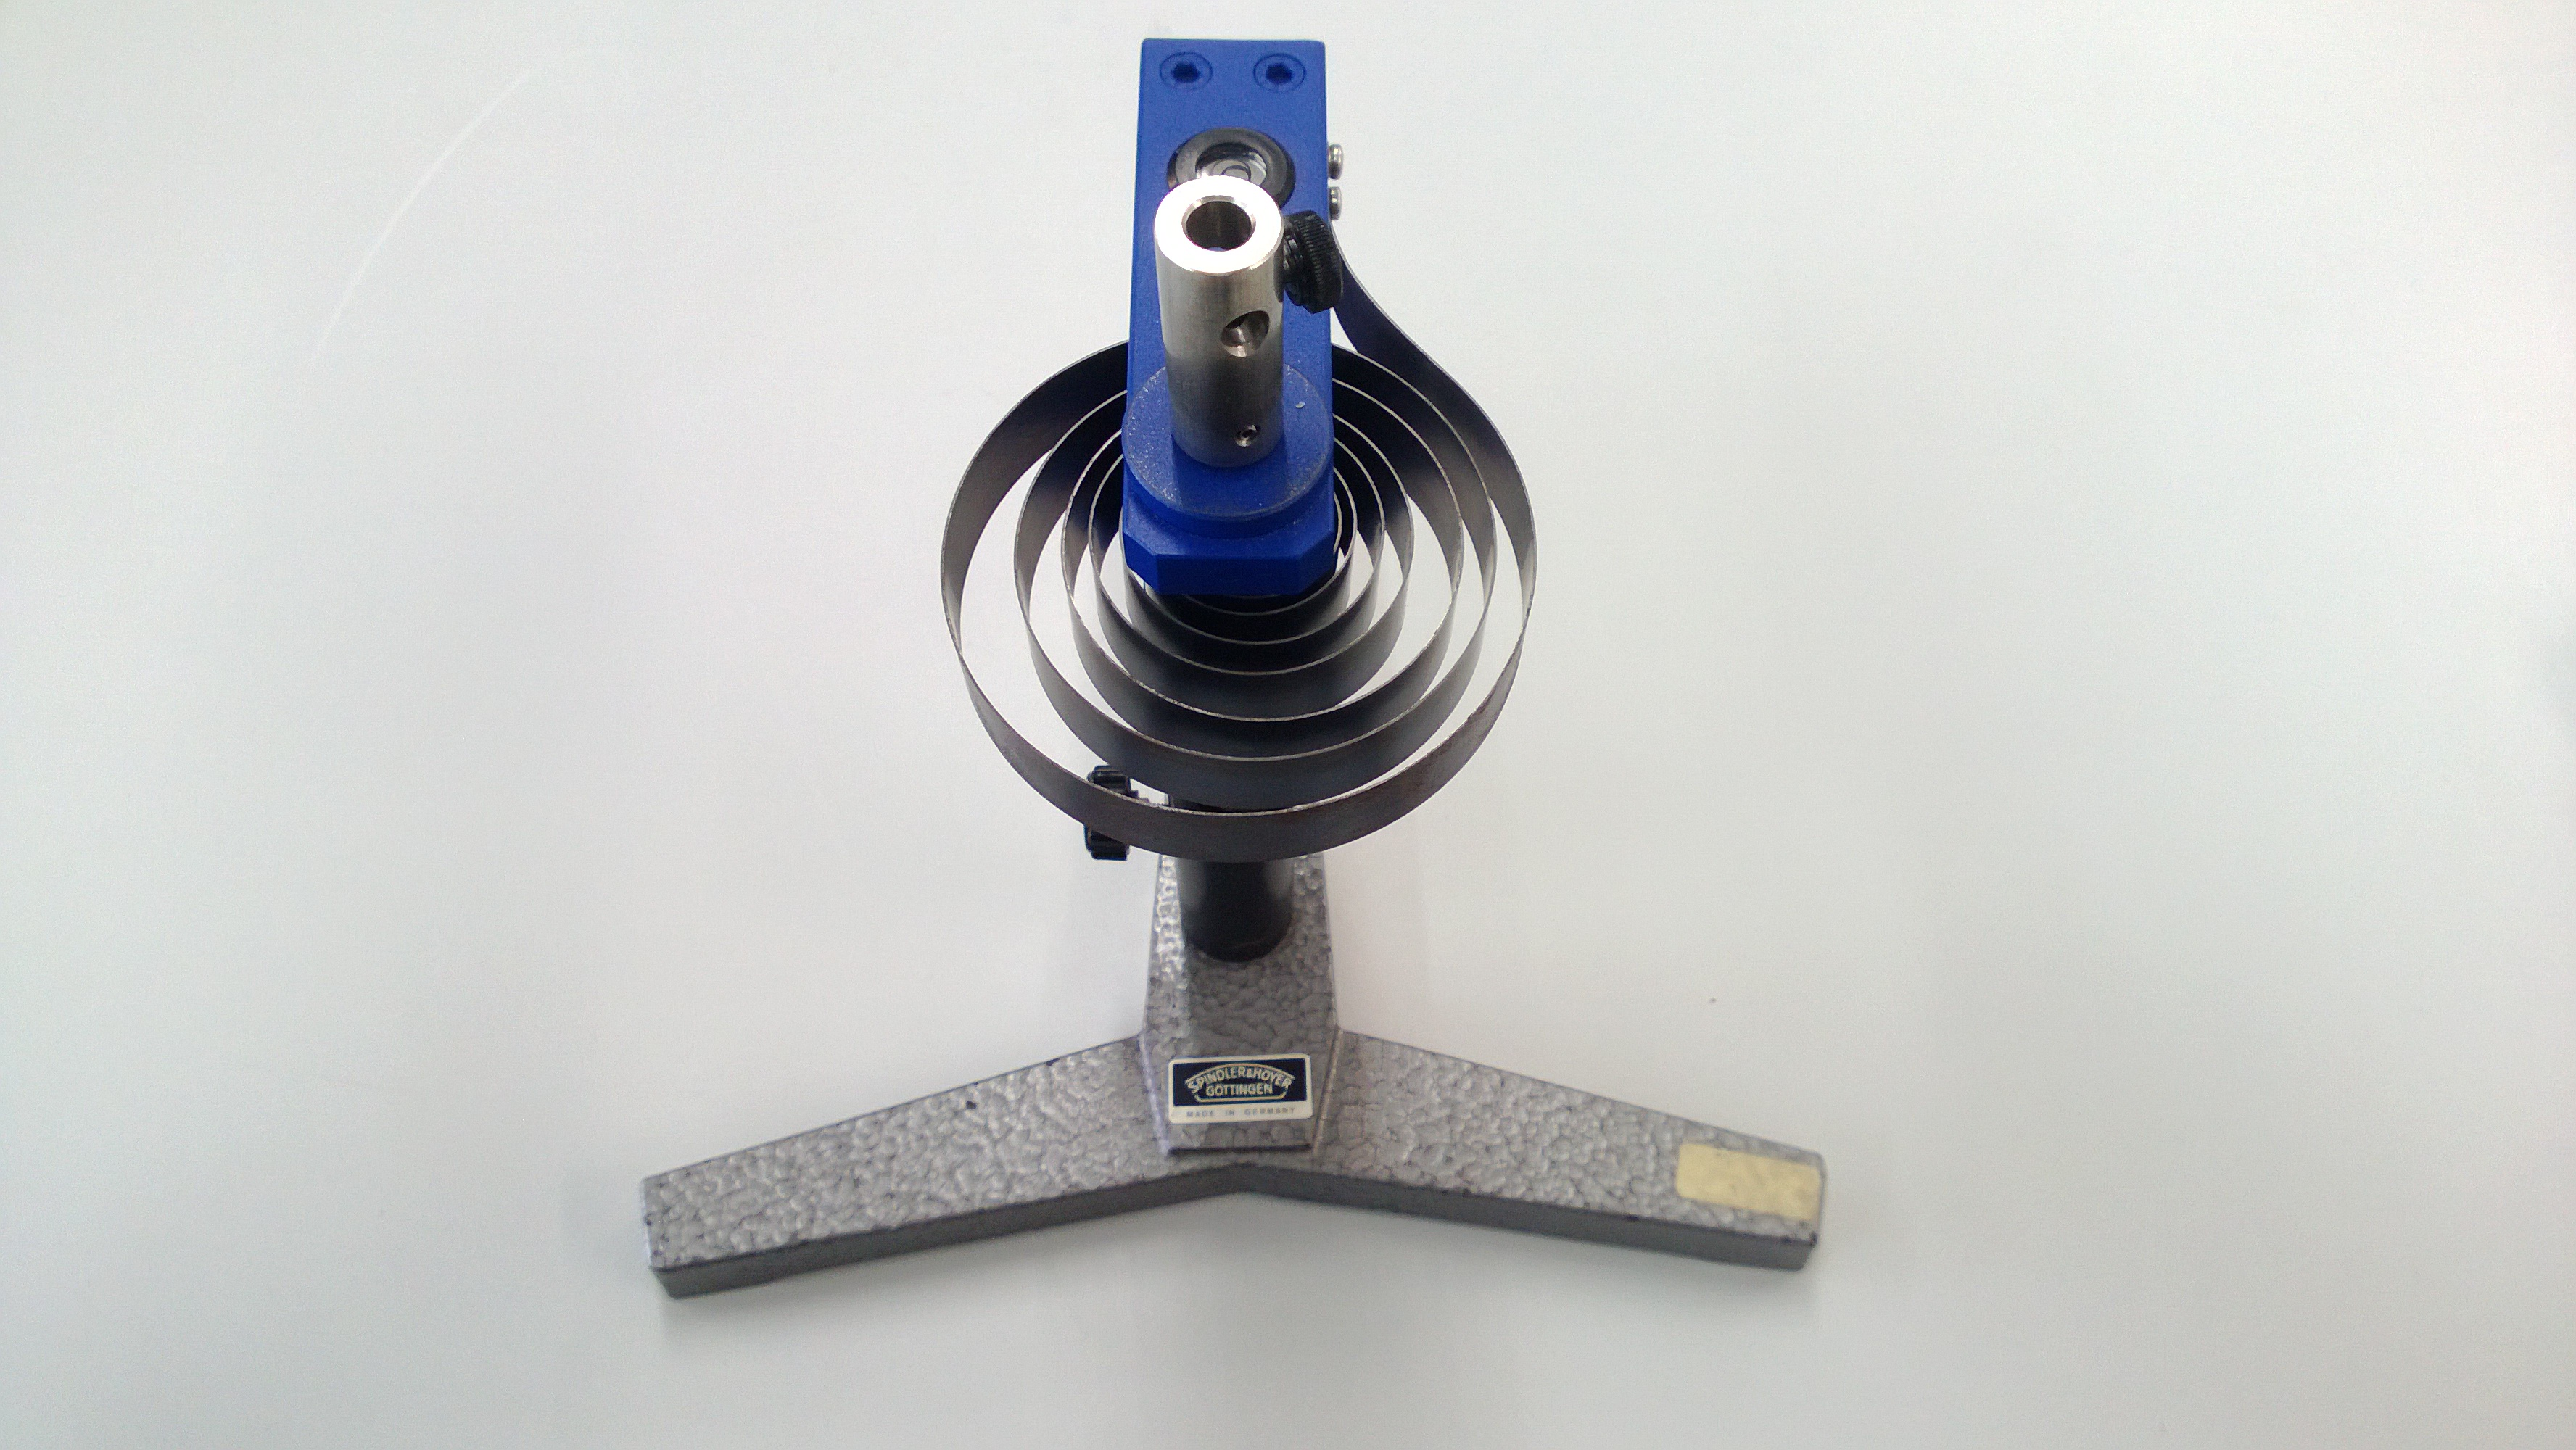
\includegraphics[scale=0.05]{content/Apparatur_1.jpg}
  \caption{Aufbau der Messapparatur}
  \label{fig:Aufbau}
\end{figure}

Zunächst wird ein Stab senkrecht zur Drehachse eingespannt und 
mit einem Kraftmesser die Kraft am Hebelarm in Abhängigkeit des 
Winkels gemessen. Es werden insgesamt 10 Kraft-Winkel Paare 
gemessen. Dabei wird darauf geachtet, dass der Kraftmesser immer
tangential zur Drehrichtung der Feder gehalten wird. Die Länge 
des Hebelarmes wird notiert. 
Anschließend werden entlang des "masselosen" Stabes zwei identische
Gewichte symmetrisch zur Drehachse angebracht. Mit Stoppuhren 
wird die Schwingungsdauer von 5 Schwingungsperioden des angeregten
Systems gemessen. Dieser Vorgang wird für 10 verschiedene Abstände 
zwischen Gewichten und Drehachsen durchgeführt. Es wird die Masse 
der verwendeten Gewichte notiert. \\
\newline
Im zweiten Versuchsteil werden eine Kugel und ein Zylinder nacheinander 
auf der Drillachse befestigt. Erneut wird das Sytem angeregt 
und die Schwingungsdauer von 5 Schwingungsperioden gemessen. 
Diese Einzelmessung wird für beide Körper insgesamt 10 mal durchgeführt.\\
\newline
Im dritten Versuchsteil wird die Messung der Schwingungsdauer einer 
Holzpuppe analog zum zweiten Teil für zwei verschiedene Stellungen 
durchgeführt. Die erste Stellung ist mit ausgestreckten Armen und die
zweite mit angezogenen Armen gegeben. Zur Modellierung 
der Puppe, werden die Beine, Arme, Torso und Kopf seperat ausgemessen. 
Dazu wird der Durchmesser und die Länge der Körper bestimmt. Zudem 
werden der Abstand von Armen und Beinen zur Drehachse und die 
Gesamtmasse der Puppe festgestellt. 